\section{平面向量的运算}

本节要点:
\begin{itemize}
    \item 掌握向量的运算的概念;
    \item 掌握向量的运算法则;
    \item 理解向量运算的几何意义。
\end{itemize}

\begin{tcolorbox}
本节将向量作为一个整体,或者说将向量作为一个一类数,定义了运算法则。下一节将向量和实数关联讨论运算法则,注意这两节的区别。
\end{tcolorbox}

本节对向量的运算做了定义,特别是内积,“6.2.4向量的数量积”定义了内积,这个概念是实数没有的,需要熟悉,把该小节的所有例题全部吃透!反复吃透!

加法的交换律和结合律:
\begin{align*}
&\boldsymbol{a}+\boldsymbol{b}=\boldsymbol{b}+\boldsymbol{a} \\
&\left( \boldsymbol{a}+\boldsymbol{b} \right) +\boldsymbol{c}=\boldsymbol{a}+\left( \boldsymbol{b}+\boldsymbol{c} \right)
\end{align*}

数乘的结合律和分配律:
\begin{align*}
&\lambda \left( \mu \boldsymbol{a} \right) =\left( \lambda \mu \right) \boldsymbol{a} \\
&\left( \lambda +\mu \right) \boldsymbol{a}=\lambda \boldsymbol{a}+\mu \boldsymbol{a} \\
&\lambda \left( \boldsymbol{a}+\boldsymbol{b} \right) =\lambda \boldsymbol{a}+\lambda \boldsymbol{b}
\end{align*}

内积的交换律和分配律,特别注意,内积没有结合律:
\begin{align*}
&\boldsymbol{a}\cdot \boldsymbol{b}=\boldsymbol{b}\cdot \boldsymbol{a} \\
&\boldsymbol{a}\cdot \left( \boldsymbol{b}+\boldsymbol{c} \right) =\boldsymbol{a}\cdot \boldsymbol{b}+\boldsymbol{a}\cdot \boldsymbol{c}
\end{align*}

两个重要的不等式:
\begin{itemize}
    \item $\left| \boldsymbol{a}+\boldsymbol{b} \right|\leqslant \left| \boldsymbol{a} \right|+\left| \boldsymbol{b} \right|$,当且仅当$\boldsymbol{a},\boldsymbol{c}$同向时等号成立;
    \item $\left| \boldsymbol{a}\cdot \boldsymbol{b} \right|\leqslant \left| \boldsymbol{a} \right|\cdot \left| \boldsymbol{b} \right|$,当且仅当$\boldsymbol{a},\boldsymbol{c}$平行时等号成立。
\end{itemize}

两个与几何相关的判断,也即数乘和内积的几何意义:
\begin{itemize}
    \item $\boldsymbol{a}=\lambda \boldsymbol{b},\lambda \ne 0\Leftrightarrow \boldsymbol{a},\boldsymbol{b}\text{平行}$;
    \item $\boldsymbol{a}\cdot \boldsymbol{b}=0\Leftrightarrow \boldsymbol{a},\boldsymbol{b}\text{垂直}$。
\end{itemize}

\begin{tcolorbox}
向量是联系代数和几何的有力工具,所以必须深刻理解向量及其运算的几何意义。向量描述了几何的点,向量的集合便是点的集合,可以构成直线、圆、弧、曲线等等。向量的运算描述了这些点和线的关系。
\end{tcolorbox}

\begin{tcolorbox}
教材从力的做功定义向量内积,略有唐突,但考虑到高中阶段背景知识也只能如此。其实向量的相乘还有一个外积,两个积合起来还有更深刻的物理意义,XML。
\end{tcolorbox}

~

\begin{example}[复习巩固7]
已知$\boldsymbol{a},\boldsymbol{b}$为两个非零向量,
\begin{enumerate}
    \item 求作向量$\boldsymbol{a}+\boldsymbol{b},\boldsymbol{a}-\boldsymbol{b}$;
    \item 当向量$\boldsymbol{a},\boldsymbol{b}$成什么位置关系时,满足$\left| \boldsymbol{a}+\boldsymbol{b} \right|=\left| \boldsymbol{a}-\boldsymbol{b} \right|$?(不要求证明)。
\end{enumerate}
\end{example}

解:

只讨论(2),直觉发现要求$\boldsymbol{a}\bot \boldsymbol{b}$。由于涉及向量的坐标表示,所以这里不要求证明,但我们在学习完6.3后回头再证明该题。
令$\boldsymbol{a}=\left( x_{\boldsymbol{a}},y_{\boldsymbol{a}} \right) ,\boldsymbol{b}=\left( x_{\boldsymbol{b}},y_{\boldsymbol{b}} \right) $,可得:
\begin{align*}
&\because \left| \boldsymbol{a}+\boldsymbol{b} \right|=\left| \boldsymbol{a}-\boldsymbol{b} \right| \\
&\therefore \left( x_{\boldsymbol{a}}+x_{\boldsymbol{b}} \right) ^2+\left( y_{\boldsymbol{a}}+y_{\boldsymbol{b}} \right) ^2=\left( x_{\boldsymbol{a}}-x_{\boldsymbol{b}} \right) ^2+\left( y_{\boldsymbol{a}}-y_{\boldsymbol{b}} \right) ^2 \\
&\therefore 2x_{\boldsymbol{a}}x_{\boldsymbol{b}}+2y_{\boldsymbol{a}}y_{\boldsymbol{b}}=-2x_{\boldsymbol{a}}x_{\boldsymbol{b}}-2y_{\boldsymbol{a}}y_{\boldsymbol{b}} \\
&\therefore x_{\boldsymbol{a}}x_{\boldsymbol{b}}+y_{\boldsymbol{a}}y_{\boldsymbol{b}}=0 \\
&\therefore \boldsymbol{a}\cdot \boldsymbol{b}=0
\end{align*}

~

\begin{example}[复习巩固12,难度:$\star $]
求证:
\[
\left( \lambda \boldsymbol{a} \right) \cdot \boldsymbol{b}=\lambda \left( \boldsymbol{a}\cdot \boldsymbol{b} \right) =\boldsymbol{a}\cdot \left( \lambda \boldsymbol{b} \right)
\]
\end{example}

解:

只证明第一个等号:
\begin{align*}
&\left( \lambda \boldsymbol{a} \right) \cdot \boldsymbol{b}=\left| \lambda \boldsymbol{a} \right|\cdot \left| \boldsymbol{b} \right|\cdot \cos \alpha =\left| \lambda \right|\cdot \left| \boldsymbol{a} \right|\cdot \left| \boldsymbol{b} \right|\cdot \cos \alpha \\
&\lambda \left( \boldsymbol{a}\cdot \boldsymbol{b} \right) =\lambda \left( \left| \boldsymbol{a} \right|\cdot \left| \boldsymbol{b} \right|\cdot \cos \alpha \right)
\end{align*}
再从$\lambda <0,>0,=0$三个方面讨论即可,略。

\begin{tcolorbox}
该关系式是内积的性质,证明性质,都从定义入手。
\end{tcolorbox}

~

\begin{example}[拓广探索23,难度:$\star $]
已知$O$为平行四边形$ABCD$所在平面内一点,且向量$\overrightarrow{OA},\overrightarrow{OC},\overrightarrow{OB},\overrightarrow{OD}$满足等式$\overrightarrow{OA}+\overrightarrow{OC}=\overrightarrow{OB}+\overrightarrow{OD}$。
\begin{enumerate}
    \item 做出满足条件的四边形$ABCD$。
    \item 四边形$ABCD$有什么特点?请证明你的猜想。
\end{enumerate}
\end{example}

\begin{figure}[h]
\centering
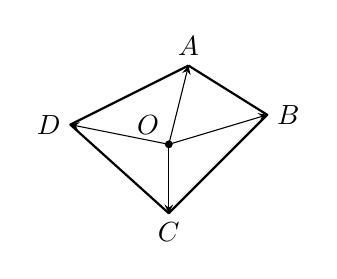
\begin{tikzpicture}[line join=round, scale=1.25]
\pgfmathparse{0.6/1.5}
\coordinate[label=above left:{$O$}] (O) at (0,0);
\coordinate[label=left:{$D$}] (D) at (-1,0.2);
\coordinate[label=right:{$B$}] (B) at (1,0.3);
\coordinate[label=below:{$C$}] (C) at (0,-0.7);
\coordinate[label=above:{$A$}] (A) at (0.2,0.8);
\fill (O) circle (\pgfmathresult mm);
\draw[thick] (A)--(B)--(C)--(D)--(A);
\draw[-stealth] (O)--(A);
\draw[-stealth] (O)--(B);
\draw[-stealth] (O)--(C);
\draw[-stealth] (O)--(D);
\end{tikzpicture}
\end{figure}

解:

$\overrightarrow{OA}+\overrightarrow{OC}$表示两向量和,但几何上起点相同,所以很难由此判断出四边形的特点,最好是首尾相连,且去掉$O$。
将等式变换化简:
\begin{align*}
&\overrightarrow{OA}+\overrightarrow{OC}=\overrightarrow{OB}+\overrightarrow{OD} \\
&\overrightarrow{OA}-\overrightarrow{OB}=\overrightarrow{OD}-\overrightarrow{OC} \\
&\overrightarrow{BO}+\overrightarrow{OA}=\overrightarrow{CO}+\overrightarrow{OD} \\
&\overrightarrow{BA}=\overrightarrow{CD}
\end{align*}
对边相等且平行,易得为平行四边形。

\begin{tcolorbox}
此题考察向量运算的几何意义,粗看较为抽象,但依然有思路可循。
\end{tcolorbox}

~

\begin{example}[拓广探索24,难度:$\star $]
如图,在$\odot C$中,是不是只需知道$\odot C$的半径或弦$AB$的长度,就可以求出$\overrightarrow{AB}\cdot \overrightarrow{AC}$的值?
\end{example}

\begin{figure}[h]
\centering
\begin{tikzpicture}[line join=round, scale=1.25]
\pgfmathparse{0.6/1.2}
\draw[thick] (0,0) circle(1);
\coordinate[label=above:{$C$}] (C) at (0,0);
\coordinate[label=left: {$A$}] (A) at (-0.72,-0.7);
\coordinate[label=right:{$B$}] (B) at (0.88,-0.47);
\fill (C) circle (\pgfmathresult mm);
\draw[-stealth] (A)--(C);
\draw[-stealth] (A)--(B);
\pic["$\alpha $",draw,angle radius=0.5cm,angle eccentricity=1.5] {angle=B--A--C};
\end{tikzpicture}
\end{figure}

解:

\begin{align*}
&\because \overrightarrow{AB}\cdot \overrightarrow{AC}=\left| \overrightarrow{AB} \right|\cdot \left| \overrightarrow{AC} \right|\cdot \cos \alpha \\
&\because \cos \alpha =\frac{\left| \overrightarrow{AC} \right|^2+\left| \overrightarrow{AB} \right|^2-\left| \overrightarrow{CB} \right|^2}{2\cdot \left| \overrightarrow{AC} \right|\cdot \left| \overrightarrow{AB} \right|} \\
&\because \left| \overrightarrow{AC} \right|=\left| \overrightarrow{CB} \right| \\
&\therefore \overrightarrow{AB}\cdot \overrightarrow{AC}=\frac{\left| \overrightarrow{AB} \right|^2}{2}
\end{align*}

略。

\begin{tcolorbox}
从向量内积的定义出发,结合余弦定理即可,非常简单。
\end{tcolorbox}




